% !TEX program = lualatex
% ECON 201, Worksheet 11: Deadweight Loss and Who Captures the Surplus.
% Compile with LuaLaTeX so the PDF is tagged. Build from the course root:
%   latexmk -lualatex -cd worksheets/worksheet11.tex && latexmk -c -cd worksheets/worksheet11.tex
% Every number here is computed and printed by slides/figures/make_lecture10.py
% (the scooter example, its own numbers rather than the deck's, read off
% the graph in figures/scooters.pdf, which the script also draws).
\DocumentMetadata{
  pdfstandard=UA-2,
  pdfversion=2.0,
  lang=en-US,
  tagging=on
}
\documentclass[11pt]{article}

\usepackage[letterpaper, margin=0.75in, top=0.5in, bottom=0.45in]{geometry}
\usepackage{fontspec}
\setmainfont{Fira Sans}
\usepackage{amsmath}
\usepackage{amssymb}
\usepackage{graphicx}
\usepackage{booktabs}
\usepackage{array}
\usepackage{xcolor}
\usepackage{needspace}
\usepackage[most]{tcolorbox}
\definecolor{cream}{HTML}{FDF3EA}
\definecolor{accent}{HTML}{BF5700}
\usepackage{titlesec}
\titleformat{\section}{\large\bfseries\color{accent}}{}{0pt}{}
\titlespacing*{\section}{0pt}{4pt}{2pt}
\usepackage{hyperref}
\hypersetup{pdftitle={ECON 201 Worksheet: Deadweight Loss and Who Captures the Surplus}, pdfauthor={Div Bhagia}, hidelinks}
\pagestyle{empty}
\setlength{\parindent}{0pt}
\setlength{\parskip}{2pt}

% Ruled answer space: n lines. Plain TeX loop; pgffor's \foreach breaks the
% enumerate counter when used inside an item.
\newcount\answerlinecount
\newcommand{\answerlines}[1]{%
  \par\vspace{1pt}\answerlinecount=#1
  \loop\ifnum\answerlinecount>0
    \rule{\linewidth}{0.3pt}\par\vspace{5pt}%
    \advance\answerlinecount by -1
  \repeat
  \vspace{-5pt}}

% Ruled grids rather than booktabs tables: students write in the cells, so
% every cell gets visible borders and the blank rows get extra height.
\newcolumntype{C}{>{\centering\arraybackslash}p{2.3cm}}
\newcommand{\blankrow}{\rule{0pt}{1.8em}}

\begin{document}

{\LARGE\bfseries\color{accent} Worksheet: Deadweight Loss}\hfill{\large ECON 201}

% Terms sit on the cream panel, where the brand orange falls below 4.5:1;
% the darker orange keeps WCAG AA contrast (see CLAUDE.md).
\definecolor{accentdark}{HTML}{8F4100}
\newcommand{\term}[1]{\textcolor{accentdark}{\textbf{#1}}}

% Definitions panel list: flush left, compact (see worksheet09).
\newenvironment{deflist}
  {\begin{list}{\textbullet}{%
     \setlength{\leftmargin}{1.1em}\setlength{\labelwidth}{0.7em}%
     \setlength{\labelsep}{0.4em}\setlength{\itemindent}{0pt}%
     \setlength{\listparindent}{0pt}\setlength{\topsep}{2pt}%
     \setlength{\partopsep}{0pt}\setlength{\parsep}{0pt}%
     \setlength{\itemsep}{2pt}}}
  {\end{list}}

\begin{tcolorbox}[colback=cream, colframe=accent, boxrule=0.6pt, arc=2pt,
  left=6pt, right=6pt, top=4pt, bottom=4pt, title=Definitions,
  fonttitle=\bfseries, coltitle=white]
\begin{deflist}
\item \term{Notation}: WTP is the buyer's willingness to pay, $P$ is the
  price, and MC is marginal cost.
\item \term{Gains from one sale}: the buyer gains $\text{WTP} - P$ and the firm
  gains $P - \text{MC}$. The \term{joint surplus} is their sum,
  $\text{WTP} - \text{MC}$.
\item \term{Pareto improvement}: a change that makes at least one person
  better off without making anyone worse off.
\item \term{Deadweight loss}: the surplus lost from sales that do not happen.
\item \term{Areas}: a triangle is $\tfrac{1}{2} \times \text{base} \times
  \text{height}$, and a rectangle is $\text{base} \times \text{height}$.
\end{deflist}
\end{tcolorbox}

\needspace{5\baselineskip}\section{Electric scooters}

A company sells electric scooters. The graph shows the demand curve for its
scooters and its marginal cost. It maximizes profit at the point $E$, where it's $MR=MC$.

\begin{center}
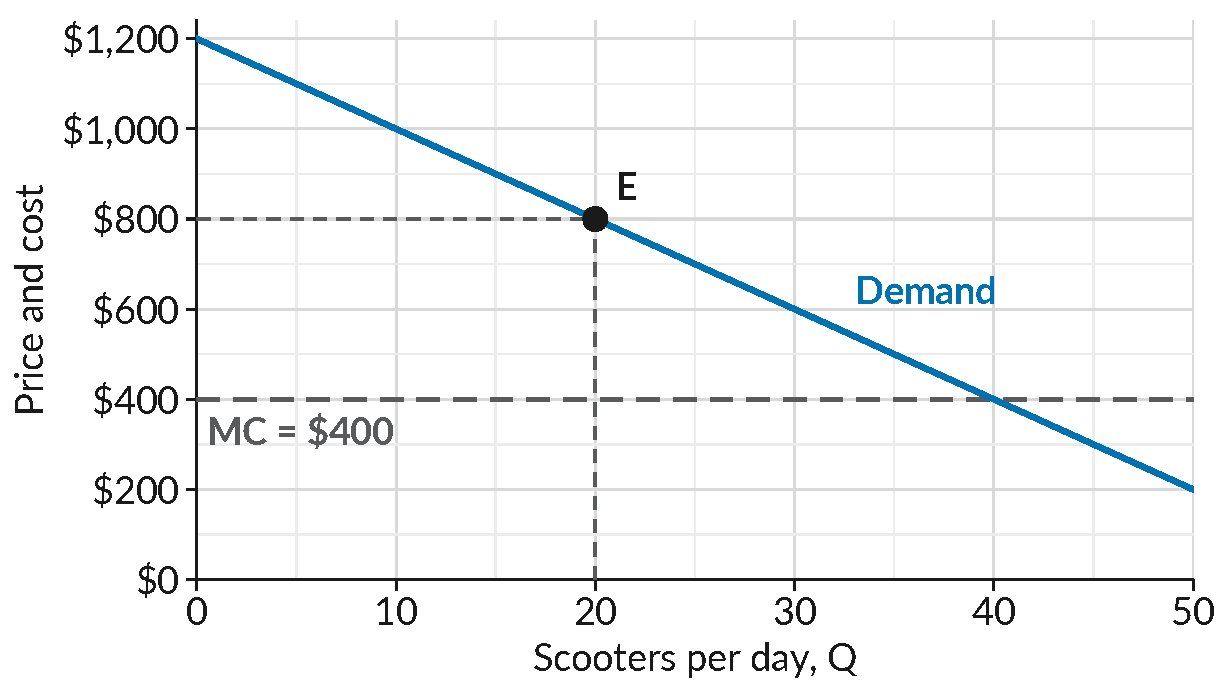
\includegraphics[width=0.72\textwidth, alt={A plotting grid, price and cost on
the vertical axis from 0 to 1,200 dollars with gridlines every 100 dollars, and
scooters per day on the horizontal axis from 0 to 50 with gridlines every 5
scooters. The demand curve falls in a straight line from 1,200 dollars at zero
scooters to zero at 60 scooters, leaving the grid at 50 scooters and 200 dollars. Marginal cost is a flat dashed line at 400
dollars. The point E is on the demand curve at 20 scooters and 800 dollars,
with dashed guides across to 800 dollars and down to 20 scooters.}]{figures/scooters.pdf}
\end{center}

\vspace{4pt}
1. How many buyers are willing to pay more than the \$400 it costs to make a
scooter? How many scooters does the company sell?
\answerlines{1}

2. How much is the 30th buyer willing to pay? Does this buyer buy at the
company's price?
\answerlines{1}

3. Suppose the company sold this buyer one scooter for \$500, and kept its price
at \$800 for everyone else. What would each side gain? Is this a Pareto
improvement?
\answerlines{2}

4. Shade the deadweight loss on the graph and find its value.
\answerlines{1}

\end{document}
